%!TEX program = xelatex
\documentclass[a4paper,12pt]{article}
	\linespread{1.3}

\usepackage{geometry} 
	\geometry{left=3cm}
	\geometry{right=1cm}
	\geometry{top=2cm}
	\geometry{bottom=2cm}

\usepackage[fleqn]{amsmath}
\usepackage{unicode-math}
\usepackage{multirow}

\usepackage[english,russian]{babel}
\usepackage{indentfirst}

\usepackage{graphicx}
	\let\ORIincludegraphics\includegraphics
	%\renewcommand{\includegraphics}[2][]{\ORIincludegraphics[scale=0.7,#1]{#2}}

\usepackage{fontspec}
	\defaultfontfeatures{Scale=MatchLowercase}
	\setmainfont[Mapping=tex-text]{Minion Pro}
	\setmonofont{Menlo}

%\usepackage{listings}
%	\lstset{
%		extendedchars=true,
%		showspaces=false,
%		showtabs=false,
%		breaklines=true,
%		showstringspaces=false,
%		breakatwhitespace=true,
%		basicstyle=\ttfamily\small
%	}
\usepackage{verbatim}

\usepackage{tabularx,booktabs}

\usepackage[nooneline]{caption}
	\captionsetup{textformat=period, figurename=Рисунок}
	\captionsetup[table]{justification=raggedright}
	\captionsetup[figure]{justification=centering} 
	\DeclareCaptionLabelSeparator{tier}{ --- }
	\captionsetup{labelsep=tier}

\usepackage{floatrow}
	\floatsetup[table]{capposition=top}

%\usepackage{pdflscape}

\usepackage{enumitem}
\makeatletter
    \AddEnumerateCounter{\asbuk}{\@asbuk}{м)}
	\makeatother
	\setlist{nolistsep}
	\renewcommand{\labelitemi}{--}
	\renewcommand{\labelitemii}{--}
	\renewcommand{\labelitemiii}{--}
	\renewcommand{\labelenumi}{\asbuk{enumi})}
	\renewcommand{\labelenumii}{\arabic{enumii})}
	\renewcommand{\labelenumiii}{\asbuk{enumiii})}

\usepackage{tikz}
	\usetikzlibrary{arrows}

\usepackage{titlesec}
	\titleformat{\chapter}[display]
	    {\filcenter}
	    {}
	    {8pt}
	    {\bfseries}{}

	\titleformat{\section}
	    {\normalsize\bfseries}
	    {\thesection}
	    {1em}{}
 
	\titleformat{\subsection}
	    {\normalsize\bfseries}
	    {\thesubsection}
	    {1em}{}

    \titlespacing*{\chapter}{0pt}{-30pt}{8pt}
	\titlespacing*{\section}{\parindent}{*4}{*4}
	\titlespacing*{\subsection}{\parindent}{*4}{*4}
	\titlespacing*{\subsubsection}{\parindent}{*4}{*4}

\usepackage{tocloft}
	\renewcommand{\cfttoctitlefont}{\hspace{0.38\textwidth} \bfseries\MakeUppercase}

\usepackage{titletoc}
	\dottedcontents{section}[1em]{}{1em}{1pc}

\addto\captionsrussian{% Replace "english" with the language you use
  \renewcommand{\contentsname}%
    {СОДЕРЖАНИЕ}%
}


\newcommand*\oline[1]{%
  \vbox{%
    \hrule height 0.5pt%                  % Line above with certain width
    \kern0.25ex%                          % Distance between line and content
    \hbox{%
      \kern-0.1em%                        % Distance between content and left side of box, negative values for lines shorter than content
      \ifmmode#1\else\ensuremath{#1}\fi%  % The content, typeset in dependence of mode
      \kern-0.1em%                        % Distance between content and left side of box, negative values for lines shorter than content
    }% end of hbox
  }% end of vbox
}


\begin{document}
	%%!TEX root = main.tex
\begin{titlepage}

\begin{center}
  Министерство образования и науки РФ \\
  Рязанский Государственный Радиотехнический Университет \\
  \vspace{0.2cm}
  Кафедра \\
  \vspace{18em}
  \Large Отчёт по лабораторной работе N  \\
  \textbf{<<>>} 
\end{center}

\vspace{14em}

\begin{flushright}
  Выполнили: \\ студент группы 041 Володин А. Д. \\
                студент группы 041 Силкин Д. В. \\
  \vspace{1.5em}
  Проверили: \\ 
             \\ 
\end{flushright}

\vspace{\fill}

\begin{center}
  Рязань 2013
\end{center}

\end{titlepage}
	\setcounter{page}{2}
	%\tableofcontents
	%\newpage
	%%!TEX root = main.tex

\begin{center}
\textbf{ВВЕДЕНИЕ}
\end{center}
\addcontentsline{toc}{section}{ВВЕДЕНИЕ}

Теория автоматов --- самостоятельный раздел математики, имеющий разнообразную проблематику и приложения.  Основными понятиями теории автоматов являются понятия абстрактного автомата и понятие композиции автоматов. Эти понятия являются разумными абстракциями реально существующих дискретных устройств --- автоматов. Понятие абстрактного автомата позволяет характеризовать устройство с точки зрения алгоритма его функционирования, т.е. алгоритма переработки информации, который оно реализует. Понятие композиции автоматов позволяет характеризовать устройство с точки зрения его структуры, иными словами, даёт представление, каким образом данное устройство построено из других, более элементарных.

Академик В.М. Глушков показал, что любое устройство обработки цифровой информации можно представить в виде совокупности двух взаимодействующих автоматов --- управляющего УА и операционного ОА (Рисунок \ref{figure:intro_pic}).

\begin{figure}[H]
	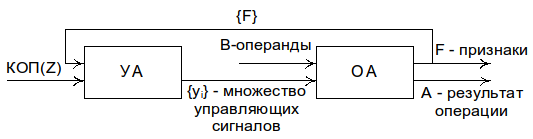
\includegraphics[scale=0.6]{images/intro.png}
	\caption{Структура цифрового автомата}
	\label{figure:intro_pic}
\end{figure}

ОА осуществляет непосредственную обработку данных путем выполнения элементарных операций над словами и выдает результат преобразования в виде двух слов: $A$ (результат) и $F$ (признаки результата, т.е. сигналы о знаках и особых значениях промежуточных и конечных результатов операций). Выполнение элементарных операций инициируется соответствующими управляющими сигналами {$y_0, y_1, y_2 ... y_m$}, которые формируются УА. 

В курсовой работе требуется разработать ОА, реализующий заданный набор арифметико-логических операций.

	%!TEX root = main.tex
\newpage
\section{Задание}



	%%!TEX root = main.tex

\newpage
%\section*{ЗАКЛЮЧЕНИЕ}
%\addcontentsline{toc}{section}{ЗАКЛЮЧЕНИЕ}
\begin{center}
\textbf{ЗАКЛЮЧЕНИЕ}
\end{center}
\addcontentsline{toc}{section}{ЗАКЛЮЧЕНИЕ}


	%%!TEX root = main.tex

\newpage

\begin{center}
\textbf{БИБЛИОГРАФИЧЕСКИЙ СПИСОК}
\end{center}
\addcontentsline{toc}{section}{БИБЛИОГРАФИЧЕСКИЙ СПИСОК}


\end{document}